\section{Experiments}\label{sec:experiments}

\begin{figure}[!t]
\centering
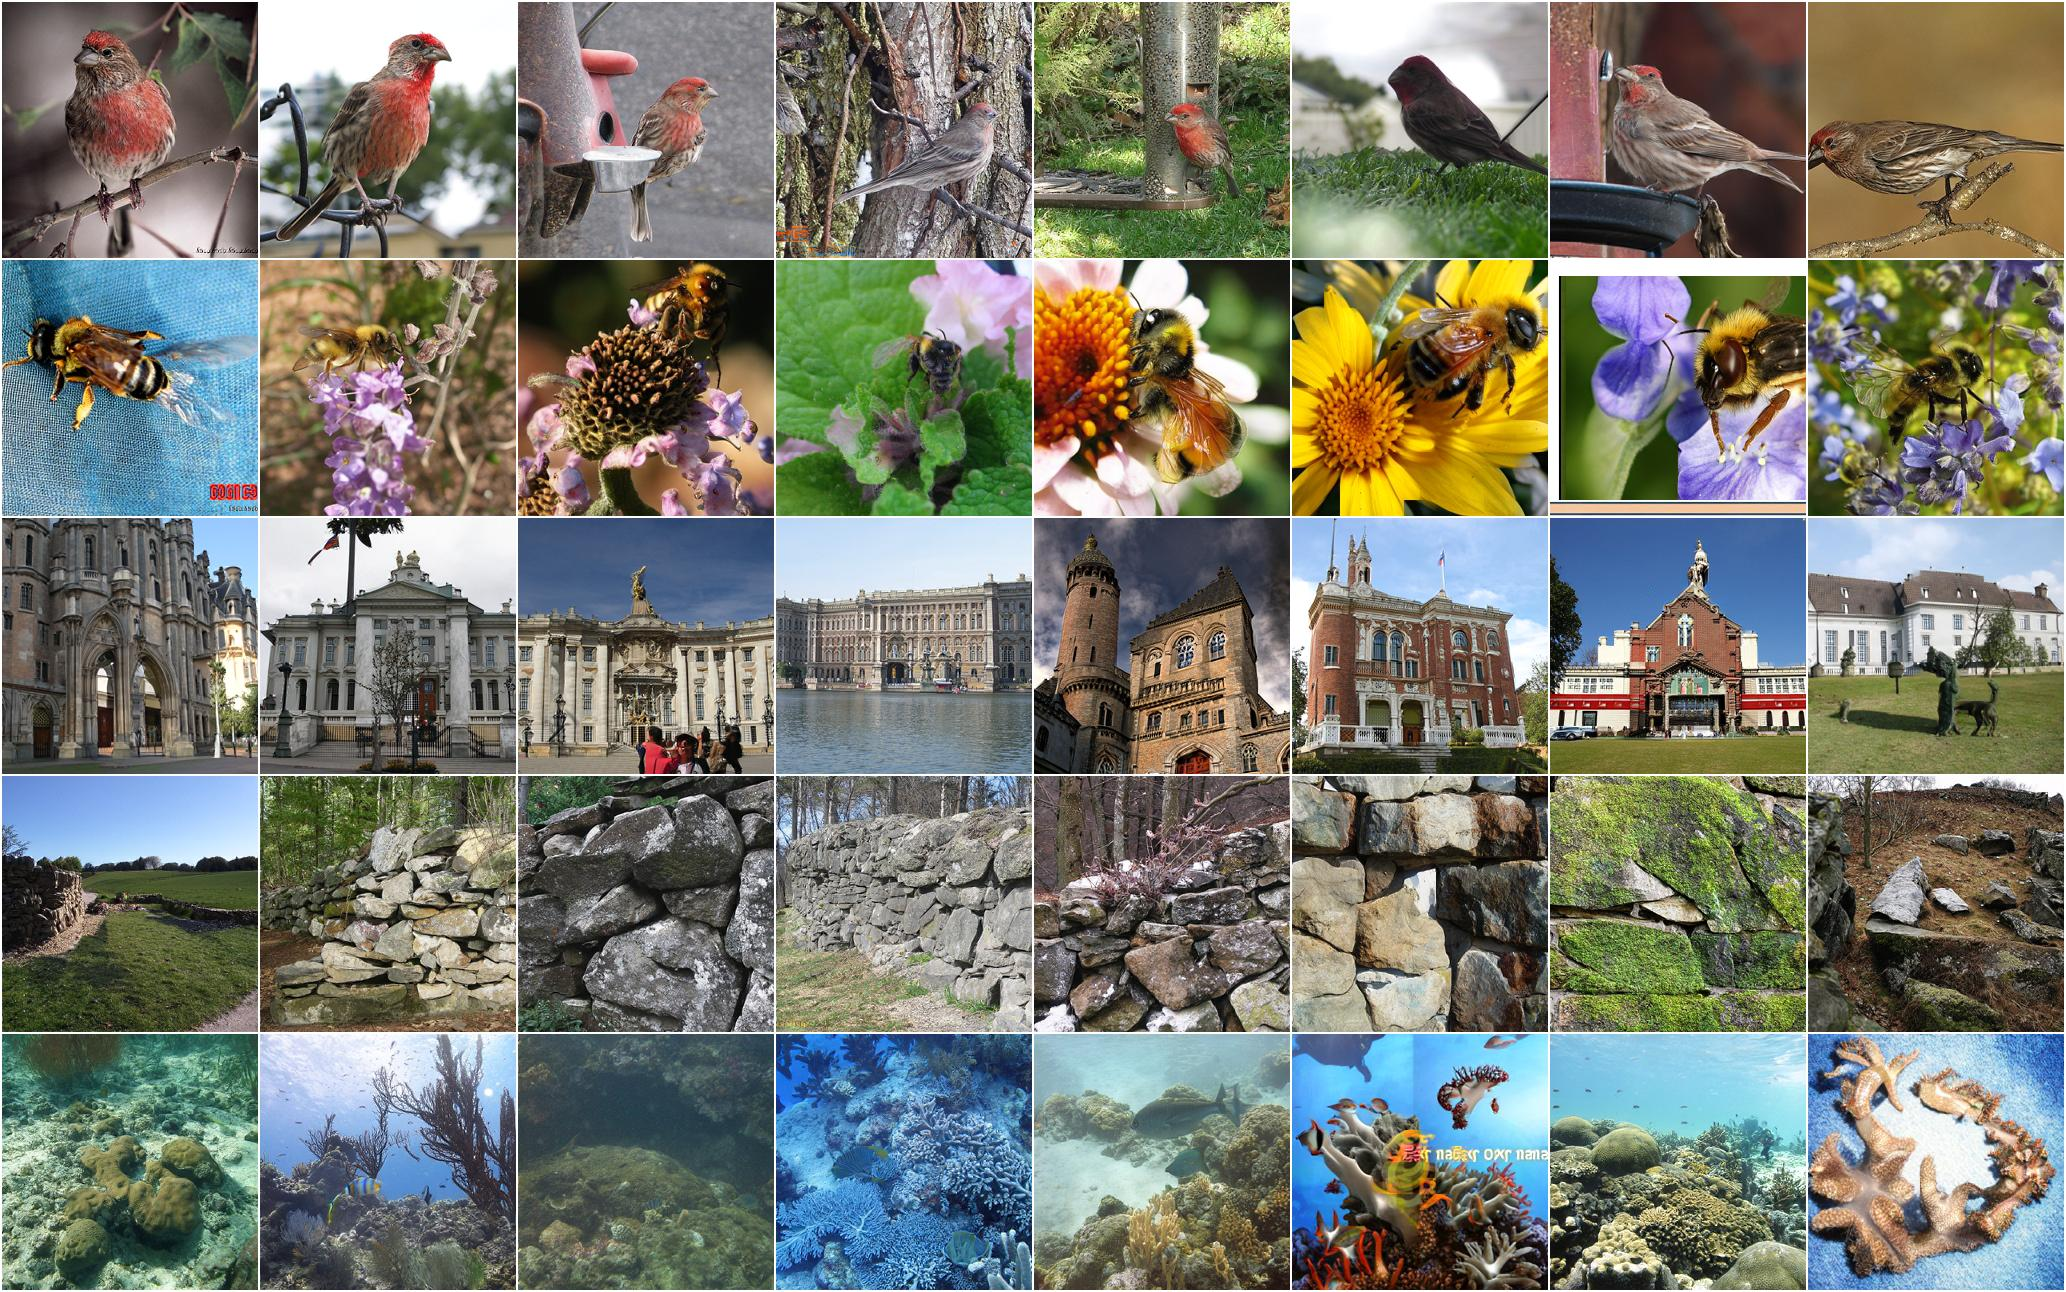
\includegraphics[width=0.9\textwidth]{imgs/combined_grid.jpg}
\caption{\textbf{Uncurated 1-NFE class-conditional samples on ImageNet $256\times256$.} Samples are generated by CrossFlow-XL from latent noise directly to pixels. Rows correspond to class 12 (house finch, linnet, \emph{Carpodacus mexicanus}), class 309 (bee), class 698 (palace), and class 973 (coral reef), respectively.}
\label{fig:imagenet_samples}
\end{figure}

We evaluate CrossFlow on ImageNet-1k~\citep{imgnet} at resolution $256\times256$. We follow the standard class-conditional protocol and report Fr\'{e}chet Inception Distance (FID)~\citep{fid} on 50,000 generated samples. The main evaluation is one-function-evaluation generation (1-NFE): the model receives a sample from the latent prior and outputs pixels directly. Unless otherwise stated, we use the linear schedule $\alpha(t)=1-t$, $\beta(t)=t$.

We implement $F_{\theta}$ with a Vision Transformer (ViT) backbone~\citep{ViT}. Following ViT conventions, we evaluate three variants: \textbf{CrossFlow-B} with 12 layers and hidden dimension 768, \textbf{CrossFlow-L} with 24 layers and hidden dimension 1024, and \textbf{CrossFlow-XL} with 28 layers and hidden dimension 1152. All models are trained using the Muon optimizer~\citep{muon,KimiMuon}, with a learning rate=8e-4 and epochs=160.

\begin{table}[t]
\centering
\caption{\textbf{System-level comparison on ImageNet $256\times256$ generation.} FID is evaluated on 50,000 generated samples. $\times 2$ in NFE indicates classifier-free guidance. Methods are grouped by sampling regime and generation space; CrossFlow is a one-step latent-to-pixel generator.}
\vspace{0.5em}
\scriptsize
\setlength{\tabcolsep}{4.5pt}
\begin{tabular}{l | cc | c | c| l | cc |c |c}
\toprule
\textbf{Method} & NFE & Space & Params & FID $\downarrow$ & \textbf{Method} & NFE & Space & Params & FID $\downarrow$\\
\midrule
\multicolumn{5}{l|}{\textit{Multi-step latent-space diffusion/flow}} & \multicolumn{5}{l}{\textit{1-NFE pixel-space GAN}}\\
\quad DiT-XL/2~\citep{dit} & 250$\times$2 & latent & 675M & 2.27 & \quad BigGAN-deep~\citep{biggan} & 1 & pixel & 56M & 6.95\\
\quad SiT-XL/2~\citep{sit} & 250$\times$2 & latent & 675M & 2.06 & \quad StyleGAN-XL~\citep{stylegan} & 1 & pixel & 166M & 2.30 \\
\quad SiT-XL/2 + REPA~\citep{repa} & 250$\times$2 & latent & 675M & \textbf{1.42} & \quad GigaGAN~\citep{gigagan} & 1 & pixel & 569M & 3.45\\
\midrule
\multicolumn{5}{l|}{\textit{Multi-step pixel-space diffusion/flow}} & \multicolumn{5}{l}{\textit{1-NFE pixel-space diffusion/flow}}\\
\quad ADM-G~\citep{adm} & 250$\times$2 & pixel & 554M & 4.59 & \quad EPG-L/16~\citep{epg} & 1 & pixel & 540M & 8.82 \\
\quad SiD, UViT~\citep{sid} & 1000$\times$2 & pixel & 2.5B & 2.44 & \quad pMF-B/16~\citep{pmf} & 1 & pixel & 118M & 3.12\\
\quad VDM++~\citep{vdmpp} & 256$\times$2 & pixel & 2.5B & 2.12 & \quad pMF-L/16~\citep{pmf} & 1 & pixel & 410M & 2.52\\
\quad SiD2~\citep{sid2} & 512$\times$2 & pixel & -- & 1.38 & \quad pMF-H/16~\citep{pmf} & 1 & pixel & 956M & 2.22 \\
\quad PixelDiT-XL/16~\citep{pixeldit} & 100$\times$2 & pixel & 797M & \textbf{1.61} \\
\midrule
\multicolumn{5}{l|}{\textit{1-NFE latent-space diffusion/flow}} & \multicolumn{5}{l}{\textbf{\textit{1-NFE latent-to-pixel (ours)}}} \\
\quad iCT-XL/2~\citep{ICT} & 1 & latent & 675M  & 34.24 & \quad CrossFlow-B & 1 & latent$\to$pixel & 95M & 2.54 \\
\quad Shortcut-XL/2~\citep{shortcut} & 1 & latent & 676M & 10.60 & \quad CrossFlow-L & 1 & latent$\to$pixel & 315M & 1.69 \\
\quad MeanFlow-XL/2~\citep{meanflow} & 1 & latent & 676M & 3.43 & \quad CrossFlow-XL & 1 & latent$\to$pixel & 461M & \textbf{1.62}\\
\quad iMF-XL/2~\citep{imf} & 1 & latent & 659M & 1.72 \\
\bottomrule
\end{tabular}
\label{tab:main_results}
\end{table}

\subsection{Main Results: 1-NFE FID}

We first evaluate one-step image generation. Table~\ref{tab:main_results} compares CrossFlow against prior ImageNet $256\times256$ results, across different representation spaces and sampling regimes.
%, the table is a system-level landscape comparison.
%including multi-step latent-space methods, multi-step pixel-space methods, one-step latent-space methods, GANs, one-step pixel-space diffusion or flow models, and our one-step latent-to-pixel setting.

Overall, CrossFlow achieves strong results with a single function evaluation.  CrossFlow-XL achieves 1.62 FID, a competitive performance with multi-step latent diffusion methods such as DiT-XL/2 (2.27 FID with 250 steps) and SiT-XL/2 (2.06 FID with 250 steps). Among the one-step methods, our CrossFlow improves over the one-step latent-space method iMF-XL/2 (1.72 FID), while avoiding a separate decoder at inference. We provide uncrated samples in Figure~\ref{fig:imagenet_samples} for a qualitative comparison.

We also demonstrate the scalability of the CrossFlow model: the FID improves from 2.54 (CrossFlow-B) to 1.62 (CrossFlow-XL) as we increase the parameters from 95M to 461M. 

%as the parameter number increases from 95M to 461 
%CrossFlow-B reaches 2.54 FID, CrossFlow-L reaches 1.69 FID, and CrossFlow-XL reaches 1.62 FID.

\begin{figure}[!t]
\centering
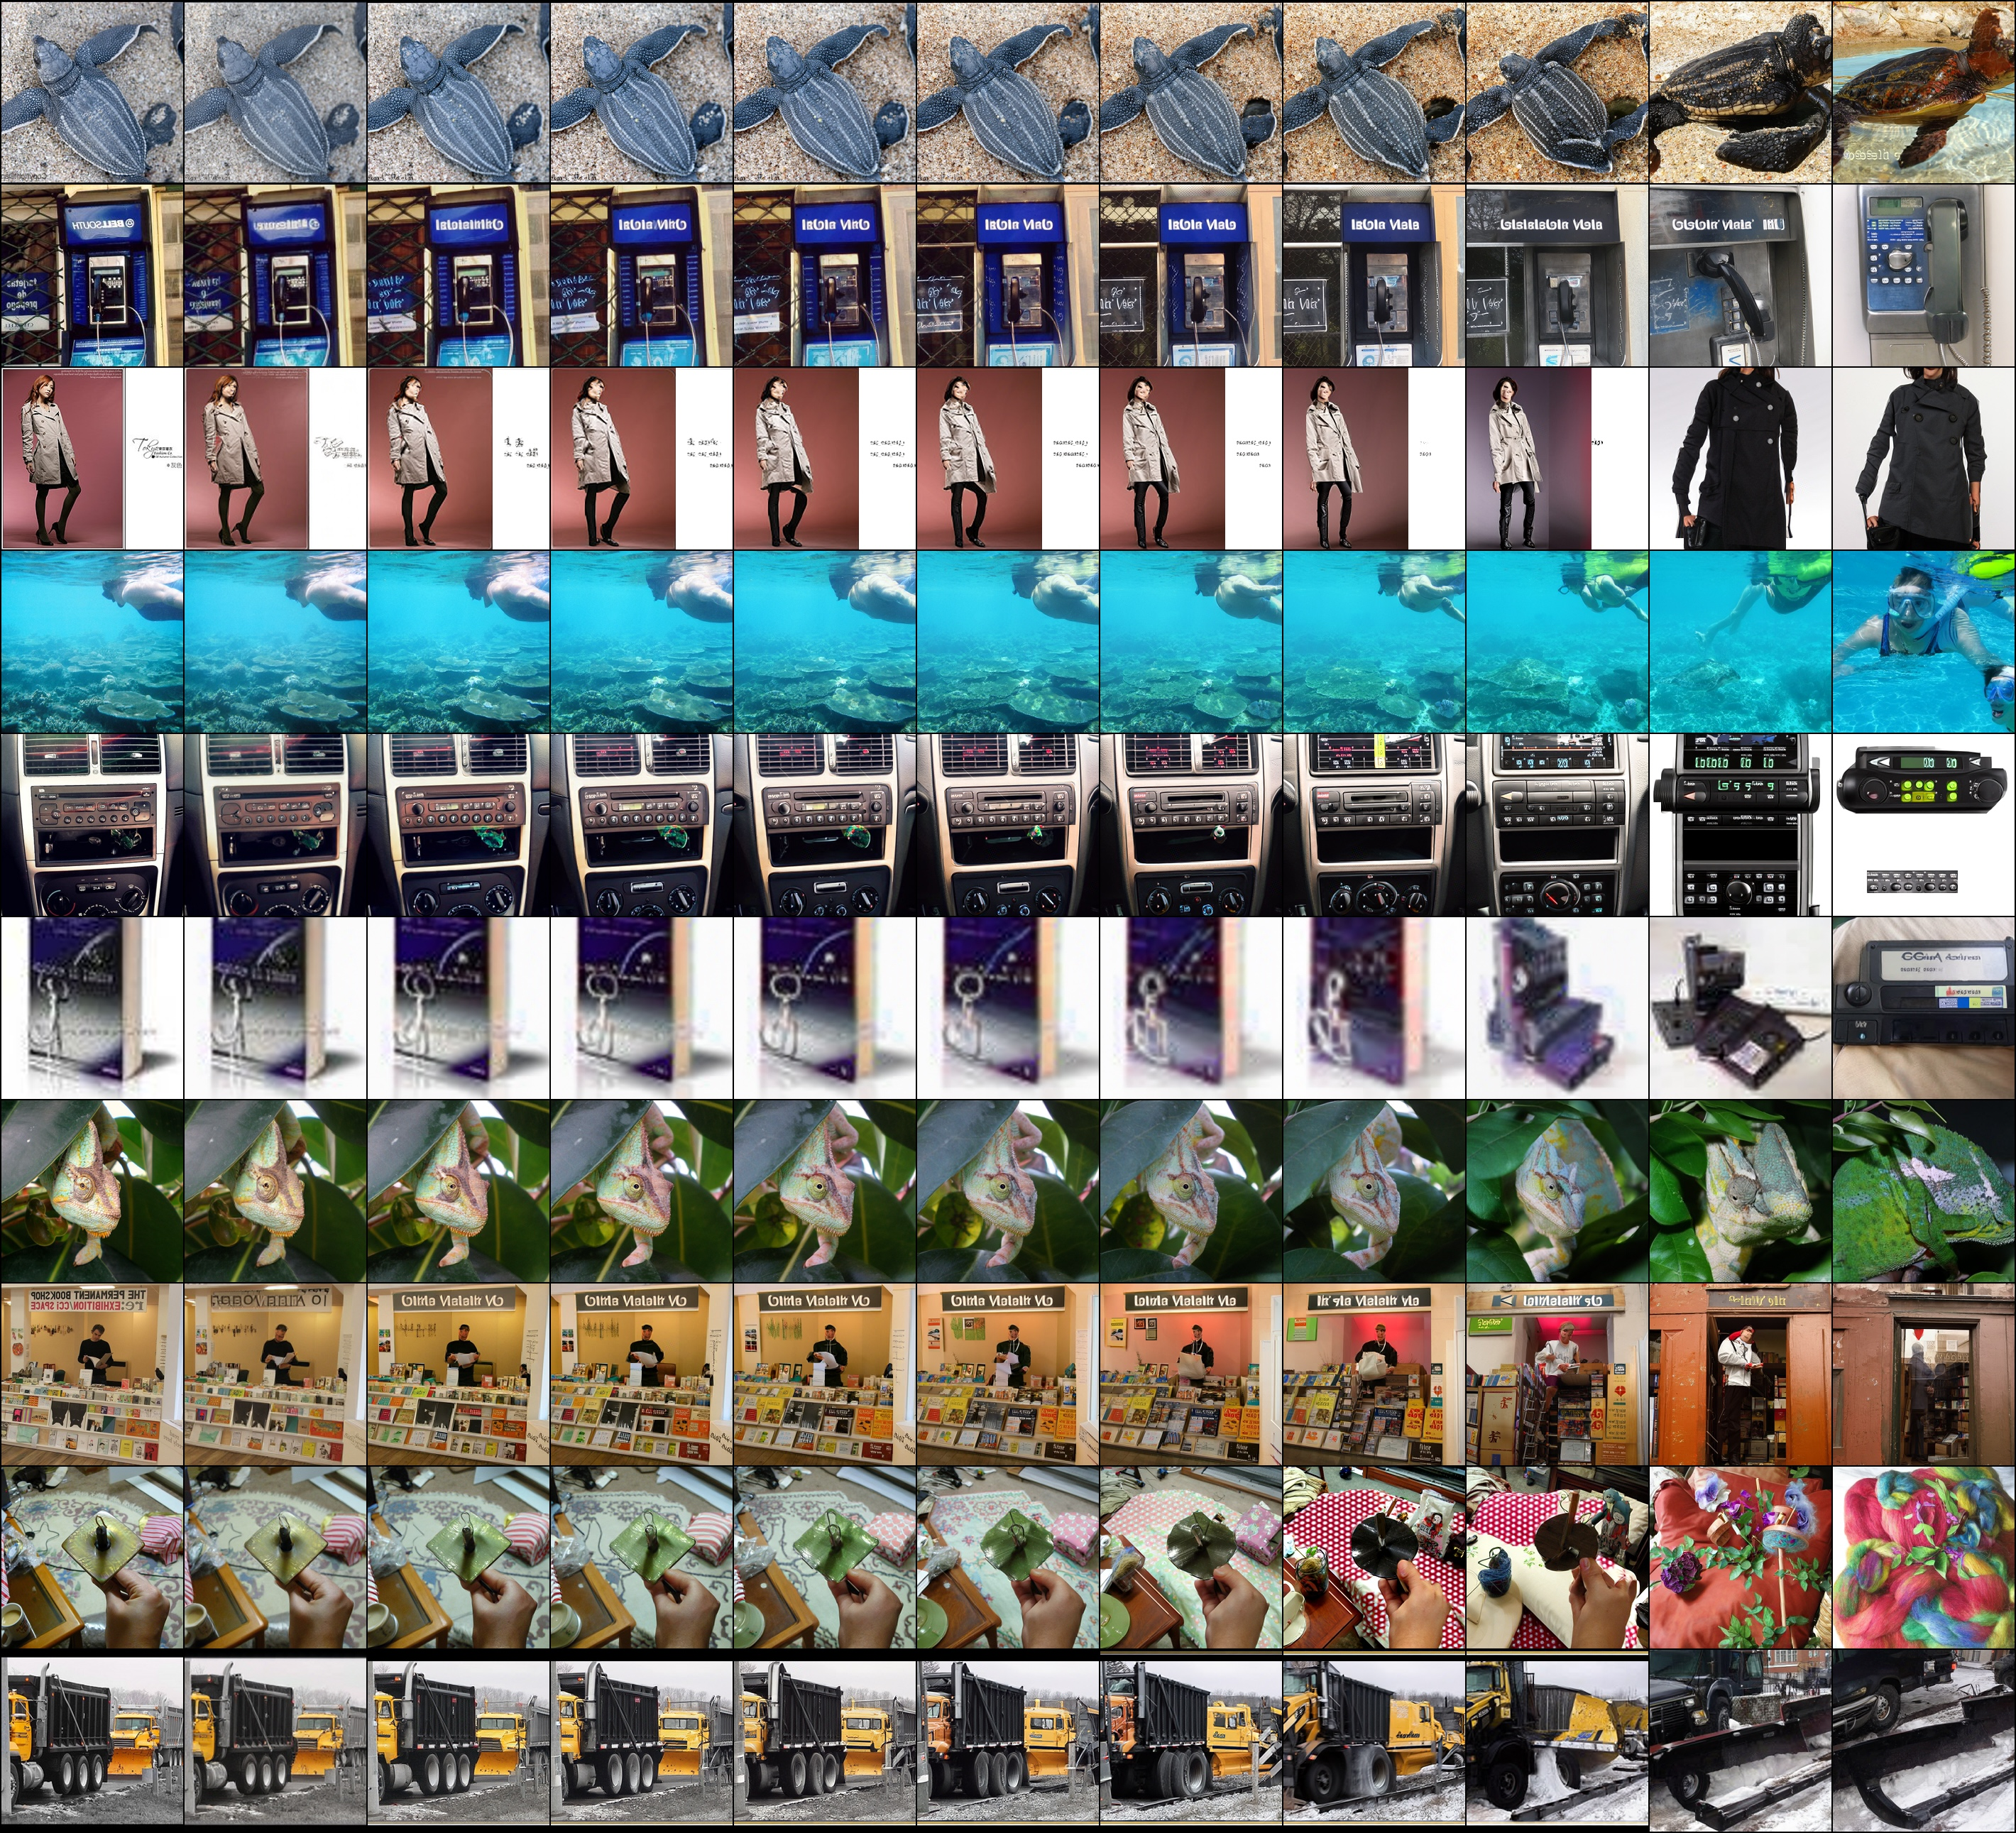
\includegraphics[trim={0 620 0 0}, clip, width=0.9\textwidth]{imgs/interp_img.jpg}
\caption{\textbf{Visualization of $F_{\theta}(z_t, t, 0)$ as $t$ varies from 0 (left, clean latent) to 1 (right, pure noise).} Each row represents a different semantic category. The interpolation preserves recognizable structure while progressively introducing stochastic variation and noise.}
\label{fig:imagenet_interp}
\end{figure}

\begin{table}[!ht]
\centering
\caption{\textbf{Ablation studies.} Unless otherwise specified, all models use CrossFlow-B, the VA-VAE encoder, the full loss configuration, the Muon optimizer, $r$-only time conditioning, no class-label dropout, and 160 training epochs.}
\vspace{0.5em}
\small
\setlength{\tabcolsep}{3pt}
\begin{tabular}{l c l c}
\toprule
\textbf{Ablation} & \textbf{FID $\downarrow$} & \textbf{Ablation} & \textbf{FID $\downarrow$}\\
\midrule
\multicolumn{2}{l}{\textit{Reference setting}} \\
Full CrossFlow-B & \textbf{2.54} \\
\midrule
\multicolumn{2}{l}{\textit{Encoder choice}} \\
Encoder: SD-VAE~\citep{ldm}, 16 latent channels & 4.08 &
Encoder: FLUX.2~\citep{flux2}, 128 latent channels & 3.81 \\
\midrule
\multicolumn{2}{l}{\textit{Auxiliary losses and objective variants}} \\
Loss: $\phi(r) = 0$ & 8.70 &
Loss: JVP with estimated marginal velocity & 7.06\\
Loss: without GAN loss & 8.86 &
Loss: without perceptual loss & 30.21 \\
Loss: without both perceptual and GAN losses & 50.65 \\
\midrule
\multicolumn{2}{l}{\textit{Training and conditioning choices}} \\
Optimizer: Muon $\rightarrow$ AdamW & 2.80 &
Time conditioning: $r\rightarrow(r,t)$ & 2.73 \\
Class conditioning: drop class labels by 10\% & 2.76 \\
\bottomrule
\end{tabular}
\label{tab:ablation}
\end{table}

\subsection{Ablation Studies}
We ablate our primary design choices using the CrossFlow-B architecture. As shown in Table~\ref{tab:ablation}, these experiments are categorized into encoder selection, auxiliary losses and objective variants, and training or conditioning configurations. Unless otherwise specified, our baseline reference setting utilizes the VA-VAE encoder, the full CrossFlow objective (including both perceptual and GAN losses), the Muon optimizer, $r$-only time conditioning, and no class-label dropout. 

\textbf{Encoder Selection.} Our framework leverages the latent space of a pretrained VAE. In this suite, we compare our default VA-VAE~\citep{VAVAE} (32 latent channels) against SD-VAE~\citep{ldm} (16 latent channels) and FLUX.2~\citep{flux2} (128 latent channels). 
The results indicate that the VA-VAE latent space yields the strongest performance, achieving an FID of 2.54, compared to 3.81 for FLUX.2 and 4.08 for SD-VAE. This trend aligns directly with the established gFID rankings of these VAEs on ImageNet-1k. These findings suggest that the specific structure of the latent representation could contribute to direct, single-step latent-to-pixel generation—though this experiment does not entirely isolate individual contributing factors, such as latent channel capacity.

\textbf{Loss and Objective Variants.} We next evaluate the impact of individual training objectives. Removing the adversarial (GAN) loss degrades the FID from 2.54 to 8.86, while omitting the perceptual loss causes a much more severe drop to 30.21. Excluding both auxiliary losses yields a poor FID of 50.65. The cross-space flow objective provides the necessary structural training signal for single-step generation, whereas the perceptual and adversarial losses act as vital regularizers that dramatically boost high-frequency sample fidelity.  

Furthermore, setting $\phi(r) = 0$ results in an FID of 8.70, and utilizing a JVP (Jacobian-Vector Product) formulation with estimated marginal velocity yields 7.06.

Crucially, these results do not imply that the core CrossFlow loss is secondary. While perceptual and GAN losses are standard staples in image VAE training~\citep{vqgan}, a traditional VAE decoder cannot natively generate samples directly from noise. The cross-space flow objective provides the necessary structural training signal for single-step generation, whereas the perceptual and adversarial losses act as vital regularizers that dramatically boost high-frequency sample fidelity. We explore the sensitivity of the GAN loss weight further in Figure~\ref{fig:gan_weight} and provide comprehensive details in Appendix~\ref{app:GANweight}.

\textbf{Training and Conditioning Choices.} The remaining ablations demonstrate that while our default optimization choices are beneficial, they are less critical to overall performance than the core loss configuration. Swapping the Muon optimizer for AdamW increases the FID to 2.80. Transitioning from $r$-only time conditioning to full $(r, t)$ conditioning yields an FID of 2.73, while introducing a 10\% class-label dropout rate results in an FID of 2.76.

\subsection{Ablation Studies}
We ablate the main design choices using CrossFlow-B. Table~\ref{tab:ablation} groups the experiments into encoder choice, objective and auxiliary losses, and training or conditioning choices. Unless otherwise specified, the reference setting uses the VA-VAE encoder, the CrossFlow objective with perceptual and GAN losses, the Muon optimizer, $r$-only time conditioning, and no class-label dropout. This organization separates representation choices from loss choices and secondary training choices, making the relative effect of each design axis easier to read.

\textbf{Encoder ablation:}. Our model leverages the encoder from a pretrained VAE. Here, we compare the performance between our default VA-VAE~\citep{VAVAE} with SD-VAE~\citep{ldm} and FLUX.2~\citep{flux2}.
The encoder ablation shows that the VA-VAE latent space gives the best result among the tested encoders. FLUX.2 reaches 3.81 FID and SD-VAE reaches 4.08 FID, compared with 2.54 FID for VA-VAE. This is consistent with the ranking of GFID of those VAE in ImageNet-1k. 
This suggests that the latent representation matters for direct one-step latent-to-pixel generation, although the experiment does not isolate a single cause, such as channel count alone.

\textbf{Loss ablation:} 
We first ablate the choice of training loss, Removing the GAN loss degrades FID from 2.54 to 8.86, while removing the perceptual loss causes a larger degradation to 30.21. Removing both auxiliary losses gives 50.65 FID. These results should not be interpreted as saying that the CrossFlow loss is incidental. Perceptual and GAN losses are common in image VAE training~\citep{vqgan}, but a standard VAE decoder cannot generate from noise. The consistency-loss baseline also shows that the cross-space flow objective is needed for one-step generation. Overall, the CrossFlow objective supplies the structural training signal, while perceptual and adversarial losses substantially improve sample fidelity. Figure~\ref{fig:gan_weight} further shows that the GAN loss weight matters; Appendix~\ref{app:GANweight} provides details.

The remaining ablations show that the default training choices are meaningful but less dominant than the objective and loss configuration. Replacing Muon with AdamW gives 2.80 FID, using $(r,t)$ time conditioning gives 2.73 FID, and dropping class labels with 10\% probability gives 2.76 FID.

\begin{minipage}[t]{1.0\linewidth}
\begin{minipage}[t]{0.48\linewidth}
    \centering
    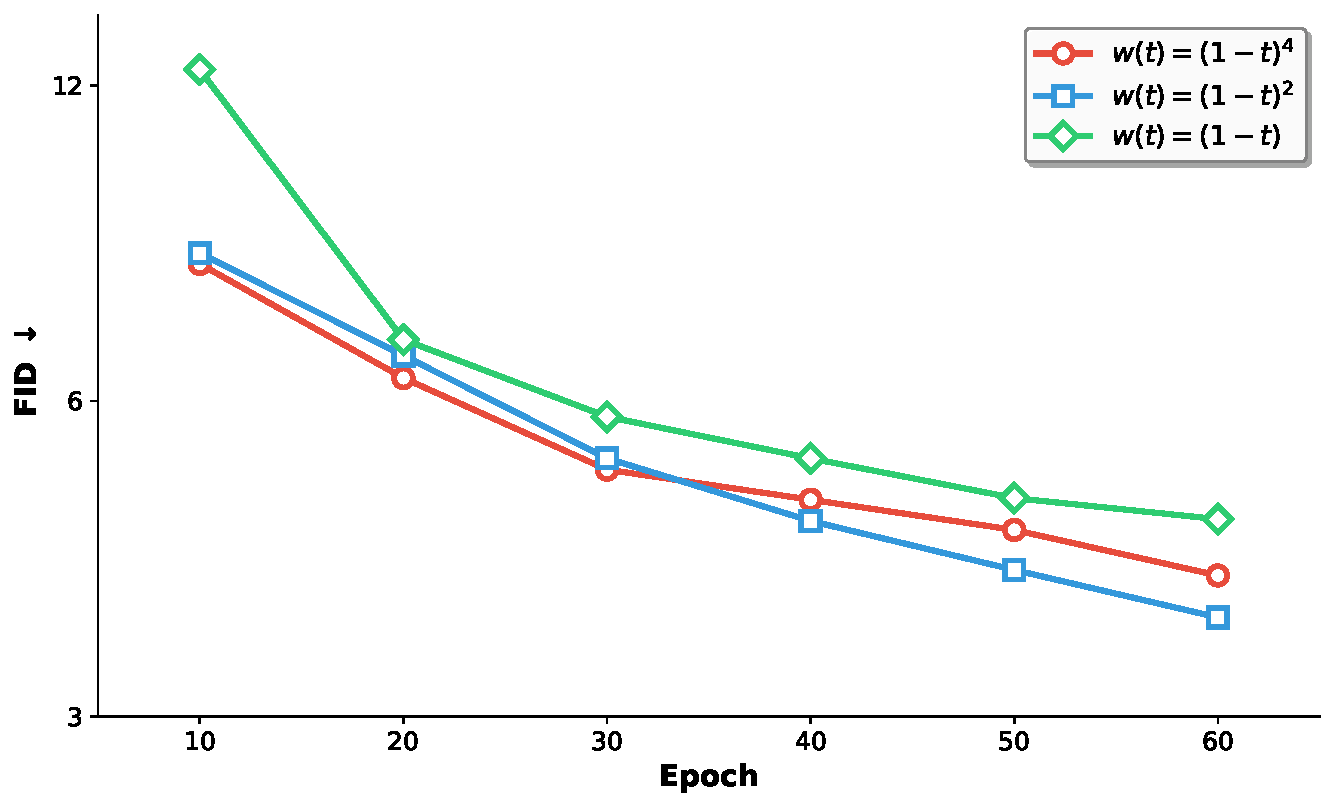
\includegraphics[width=1.0\linewidth]{imgs/plot_ganleak.pdf}
    \captionof{figure}{\textbf{Ablation of the GAN weight scheduler $w(t)$.} Higher GAN weights lead to higher FID because of partial mode collapse, while overly small weights on high-noise latents slow initial convergence. The optimized schedule balances stability and convergence speed.}
    \label{fig:gan_weight}
\end{minipage}
\hfill
\begin{minipage}[t]{0.48\linewidth}
    \centering
    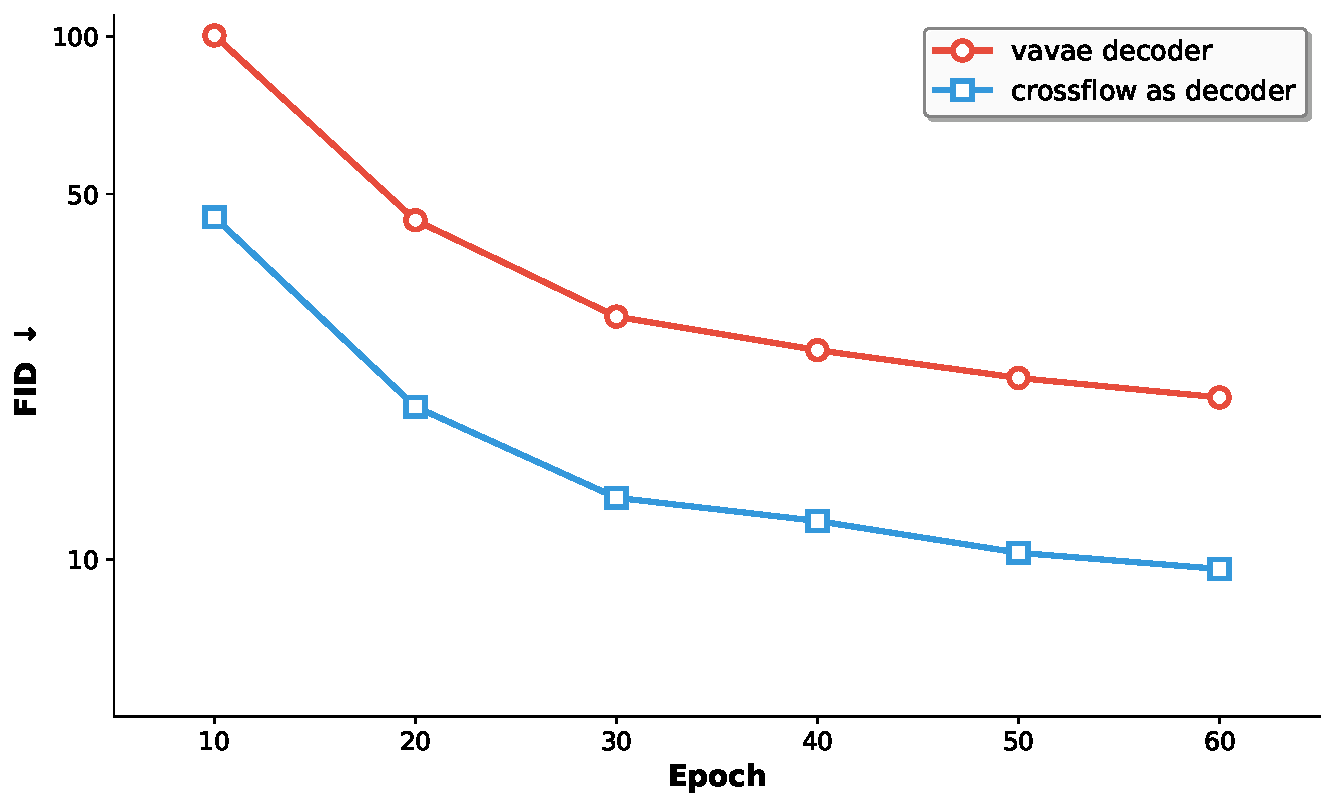
\includegraphics[width=1.0\linewidth]{imgs/plot_dit.pdf}
    \captionof{figure}{\textbf{CrossFlow as a VAE decoder.} We evaluate CrossFlow as a VAE decoder for latent diffusion and report FID over training epochs for a LightningDiT-B/1 generator in the VA-VAE latent space. CrossFlow consistently improves generation quality over the VA-VAE decoder.}
    \label{fig:crossflow_vae}
\end{minipage}
\end{minipage}

\subsection{Performance as a VAE Decoder}

Finally, we evaluate CrossFlow as a decoder in a VAE-style pipeline. This setting tests whether the same latent-to-pixel model can serve not only as a generator, but also as a high-quality decoder for latents produced by a latent generator. We train LightningDiT-B/1 in the VA-VAE latent space~\citep{VAVAE}. Figure~\ref{fig:crossflow_vae} compares the same DiT generator with different decoders as training progresses. CrossFlow used as a VAE decoder improves FID throughout training, supporting the claim that the model can decode generator-produced latents more effectively than the default VA-VAE decoder in this setting.
